              %*****************************************************************%
              %                                                                 %
              %         Adapted from a thesis model by Lorenzo Pantieri         %
              %                       Alessandro Candido                        %
              %                                                                 %
              %                                                                 %
              %*****************************************************************%
       
% !TEX encoding = UTF-8 Unicode
% !TEX root = thesis.tex
% !TEX spellcheck = en-US

\documentclass[11pt,%                      % corpo del font principale
               a4paper,%                   % carta A4
               twoside,openright,%         % fronte-retro
%              oneside,openany,%           % solo fronte
               titlepage,%                 % frontespizio
               headinclude,,footinclude,%  % testatina e piede di pagina
               BCOR=5mm,%                   % rilegatura di 5 mm
               cleardoublepage=empty,%     % pagine vuote senza testatina e piede di pagina
               captions=tableheading,%     % didascalie in cima alle tabelle
               ]{scrreprt}                 % classe report di KOMA-Script;
               
% !TEX encoding = UTF-8
% !TEX root = ../thesis.tex

% font encoding:
% NOTA BENE! richiede una distribuzione *completa* di LaTeX,
% per esempio TeXLive o MiKTeX *complete*
\usepackage[T1]{fontenc}

% input encoding:
% [latin1] is also fine
% ACHTUNG! Sync to editor preferences
\usepackage[utf8]{inputenc}

% to write both in Italian and English;
% last language is the default one
\usepackage[italian,english]{babel}

% frontespizo
% per includerlo nel documento bisogna:
% 1. compilare una prima volta Tesi.tex;
% 2. compilare a parte Tesi-frn.tex, generato dalla compilazione precedente;
% 3. compilare ancora Tesi.tex.
%\usepackage[suftesi]{frontespizio}


 % rientra il primo capoverso di ogni sezione
\usepackage{indentfirst}

% images
\usepackage{graphicx}

% codes
\usepackage{listings}

% quotes
\usepackage[font=small]{quoting}

% math
\usepackage{amsmath,amssymb,amsthm}

% complete page references
\usepackage[english]{varioref}

% fixed width tables
\usepackage{tabularx}

% double quotes optimized for biblatex
\usepackage[autostyle,italian=guillemets]{csquotes}

% bibliography;
% make citing style author-year;
% the style "numeric-comp" makes numeric references;
\usepackage[style=philosophy-modern, url=false,
			hyperref,square,backend=biber]{biblatex}

% biblatex database
\addbibresource{library.bib}

% sub-figures and sub-tables
\usepackage{subfig}

% pseudo-text
\usepackage{lipsum}

% ClassicThesis style
% - chapter numbers in Euler font
% - if using subfig package
% - Bera Mono as monospace font
% - AMS Euler as math font
% - improve line spacing
% - codes
% - for documents divided in parts 
\usepackage[eulerchapternumbers,%
            subfig,%
            beramono,%
            eulermath,%
            pdfspacing,%
            listings,%
            parts,%
            ]{classicthesis}
% rearrange the appearance of classicthesis
\usepackage{arsclassica}

% inner=2.5cm,
\usepackage[bottom=3.5cm]{geometry}

\newlength{\myshift}
\setlength{\myshift}{4mm}
\addtolength{\evensidemargin}{-\myshift}
\addtolength{\oddsidemargin}{\myshift}
%\setlength{\evensidemargin}{8.40024mm} % initial value: 12.40024mm
%\setlength{\oddsidemargin}{3.80026mm} % initial value: -0.19974mm

% grey-scale
\usepackage{ifthen}
\newboolean{gs}
\setboolean{gs}{false}

% personal settings
% Here are stored personal settings

%*********************************************************************************
% Personal commands
%*********************************************************************************
% author
\newcommand{\myName}{Alessandro Candido}                        
% title
\newcommand{\myTitle}{Theory Predictions for PDF fitting}
% thesis type
\newcommand{\myDegree}{PhD Thesis}                          
% university
\newcommand{\myUni}{Universit\`a degli Studi di Milano}       					
% department
\newcommand{\myDepartment}{Dipartimento di Fisica Aldo Pontremoli}      
% supervisor
\newcommand{\myProf}{Prof.~Stefano Forte}             		
% co-supervisor
\newcommand{\myOtherProf}{Prof.~Stefano Carrazza}        
% where
\newcommand{\myLocation}{Milan}                                  
% when
\newcommand{\myTime}{\DTMMonthname{\the\month} \the\year}       

%*********************************************************************************
% amsmath, amssymb, amsthm settings
%*********************************************************************************

% theorem, laws, and acts (amsthm package required)
\theoremstyle{plain} 
\newtheorem{theorem}{Theorem}
\newtheorem{law}{Law}
\newtheorem{act}[law]{Act}
\newtheorem{murphy}{Murphy}[section]

%*********************************************************************************
% biblatex settings
%*********************************************************************************
\defbibheading{bibliography}{%
\cleardoublepage
\manualmark
\phantomsection 
\addcontentsline{toc}{chapter}{\tocEntry{\bibname}}
\chapter*{\bibname\markboth{\spacedlowsmallcaps{\bibname}}
{\spacedlowsmallcaps{\bibname}}}}

%*********************************************************************************
% listings settings
%*********************************************************************************
\lstset{language=[LaTeX]Tex,%C++,
    keywordstyle=\color{RoyalBlue},%\bfseries,
    basicstyle=\small\ttfamily,
    %identifierstyle=\color{NavyBlue},
    commentstyle=\color{Green}\ttfamily,
    stringstyle=\rmfamily,
    numbers=none,%left,%
    numberstyle=\scriptsize,%\tiny
    stepnumber=5,
    numbersep=8pt,
    showstringspaces=false,
    breaklines=true,
    frameround=ftff,
    frame=single
} 

%*********************************************************************************
% graphicx settings
%*********************************************************************************
\graphicspath{{pictures/}}

%*********************************************************************************
% Optimized margins for A4
%*********************************************************************************
\areaset[current]{370pt}{750pt}
\setlength{\marginparwidth}{7em}
\setlength{\marginparsep}{2em}%

%*********************************************************************************
% varioref settings
%*********************************************************************************
\makeatletter
\vref@addto\extrasitalian{%
   \def\reftextfaraway#1{a pagina~\pageref{#1}}%
}
\makeatother

%*********************************************************************************
% More
%*********************************************************************************

% [...] ;-)
\newcommand{\omissis}{[\dots\negthinspace]}

% hyphenation exceptions
\hyphenation{Fortran ma-cro-istru-zio-ne nitro-idrossil-amminico}

% correct scrreprt's bug about figure numbering
\renewcommand*{\figureformat}{%
  \figurename~\thefigure%
  %\autodot%
}
\renewcommand*{\tableformat}{%
  \tablename~\thetable%
  %\autodot%
}

% further styles
% !TEX encoding = UTF-8
% !TEX root = ../thesis.tex
% !TEX spellcheck = en-US

\usepackage{datetime2}
\usepackage{datetime2-calc}
\usepackage{ifthen}
\usepackage{etoolbox}
\usepackage{calc}
\usepackage[sort]{cleveref}

% glossaries (after hyperref)
\usepackage[acronym,automake,nomain,section=section]{glossaries}
%\newglossary*{sym}{Symbols}
\newglossary*{symbols}{Symbols}
\renewcommand*{\glstextformat}[1]{\textcolor{CTurl!30!black}{#1}} %color defined by classichthesis
\makeglossaries

\usepackage{ifoddpage}
% !TeX root = ../main.tex

% manage layouts
\usepackage{geometry}

% indent first paragraph of each section
\usepackage{indentfirst}

% fixed width tables
% \usepackage{tabularx}

\usepackage{booktabs}
\usepackage{subfig}
\usepackage[bottom]{footmisc}
\usepackage{float}
%\usepackage[bottom]{footmisc}		% note a fondo pagina
%\usepackage{emptypage}
\usepackage{verbatim}
\usepackage{lipsum}
\usepackage{enumerate}
%\usepackage{enumitem}
\usepackage{changepage}
\let\checkmark\relax
\usepackage{dingbat}
\usepackage{lettrine}

%*********************************************************************************
% Color Boxes
%*********************************************************************************
%\usepackage{layouts}
%\printinunitsof{mm}{\pagevalues}
%\verb|\marginparwidth|: \printinunitsof{mm}\prntlen{\marginparwidth}

%*********************************************************************************
% Tikz
%*********************************************************************************
\usepackage{pgf}
\usepackage{tikz}
\usepackage{rotating}
\usepackage{pgfornament}
% \usepackage{pgfornament,pgfornament-han}
\usetikzlibrary{arrows,shapes,decorations,automata,backgrounds,petri,positioning}

\setlength{\skip\footins}{15pt}

%*********************************************************************************
% Color Boxes
%*********************************************************************************

\usepackage{tcolorbox}
\tcbuselibrary{theorems}

%*********************************************************************************
% Optimized margins for B5
%*********************************************************************************
\KOMAoptions{BCOR=10mm}
\areaset[current]{360pt}{650pt}
\setlength{\marginparwidth}{7em}
\setlength{\marginparsep}{2em}%

%*********************************************************************************
% Minitoc settings
%*********************************************************************************
\usepackage{minitoc}
\dominitoc[e]
\mtcsetrules{minitoc}{off}
\mtcsetfeature{minitoc}{before}{\textcolor{black!70}{\rule{0.8\textwidth}{0.1pt}}\vspace{-20pt}}
\mtcsetfeature{minitoc}{after}{\vspace{-20pt}\textcolor{black!70}{\rule{0.8\textwidth}{0.1pt}}}
\setcounter{tocdepth}{2}

%*********************************************************************************
% listings settings - code snippets
%*********************************************************************************
\usepackage{listings}
\lstset{language=[LaTeX]Tex,%C++,
    keywordstyle=\color{RoyalBlue},%\bfseries,
    basicstyle=\small\ttfamily,
    %identifierstyle=\color{NavyBlue},
    commentstyle=\color{Green}\ttfamily,
    stringstyle=\rmfamily,
    numbers=none,%left,%
    numberstyle=\scriptsize,%\tiny
    stepnumber=5,
    numbersep=8pt,
    showstringspaces=false,
    breaklines=true,
    frameround=ftff,
    frame=single
} 

% !TeX root = ../main.tex

% --- PACKAGES ---
\usepackage{mathtools,physics,tensor}
\usepackage{bbold,mathrsfs}
\usepackage{bm}
\usepackage{slashed}
%\usepackage[mathscr]{euscript}
%\usepackage{bickham}		% redefines \mathcal e \mathbcal
							% al momento non riesco a farlo funzionare
%\usepackage{mathalfa}		% powerful package with a lot of math fonts
%\usepackage{fourier}		% alternativa decente a bassa sbatta
%\usepackage[euler-digits,euler-hat-accent]{eulervm}
\usepackage[cdot, thickqspace, squaren]{SIunits}
% ------------

% --- THEOREMS ---
% theorems (with amsthm) in english
\theoremstyle{plain}% default
\newtheorem{thm}{Theorem}[section]
\newtheorem{lem}[thm]{Lemma}
\newtheorem{prop}[thm]{Proposition}
\newtheorem*{thm*}{Theorem}
\newtheorem*{lem*}{Lemma}
\newtheorem*{prop*}{Proposition}
\newtheorem*{cor}{Corollary}

\theoremstyle{definition}
\newtheorem{defn}{Definition}[section]
\newtheorem{es}{Example}[section]
\newtheorem{ex}{Exercise}[section]
\newtheorem*{defn*}{Definition}
\newtheorem*{es*}{Example}
\newtheorem*{ex*}{Exercise}
\newtheorem*{note}{Note}

% ENVIRONMENTS
\newtcbtheorem[number within=section]{example}{Example}%
{colback=CornflowerBlue!4,colframe=CornflowerBlue!60!black,fonttitle=\bfseries,before upper={\parindent15pt\noindent}}{th}

%\newtcbtheorem[number within=section]{mytheo}{My Theorem}%
%{colback=green!5,colframe=green!35!black,fonttitle=\bfseries}{th}
% ------------


% mycommands
\newcommand{\ttmp}[1]{\textit{\textcolor{violet}{#1}}}
\newcommand{\gsym}[1]{\glssymbol{#1}}

%\newcommand{\Section}[2][]{
%	\ifstrempty{#1}{%
%		\section{#2}
%	}{%
%		\setcounter{section}{#1-1}
%		\section{#2}
%	}%
%}


\begin{document}
\pagestyle{scrheadings}
%******************************************************************
% Materiale iniziale
%******************************************************************
% !TeX root = ../../main.tex

\pdfbookmark{Cover}{Cover}
\newgeometry{width=370pt,height=650pt,centering}

\begin{center}
	
\includegraphics[width=11cm]{logo-unimi}
	\vspace*{10pt}

	Scuola di Dottorato in Fisica, Astrofisica e Fisica Applicata\\
	\myDepartment\\
	\vspace*{5pt}
	\textbf{Ciclo XXXV}

	\vfill

	{\Huge \myTitle}\\
	\vspace*{30pt}
	\textit{Settore Scientifico Disciplinare FIS/02}\\

	\vfill

	\textbf{Supervisor:} \hfill \textbf{Candidate:}\\
	\myProf \hfill \myName\\
	\vspace*{15pt}
	Anno Accademico 2021/2022
\end{center}
	
	
\pagenumbering{gobble}

\cleardoublepage
\restoregeometry
 
\pagenumbering{roman}
% !TEX encoding = UTF-8
% !TEX root = ../../main.tex
% !TEX spellcheck = en-US

%*******************************************************
% Frontespizio
%*******************************************************
	
\restoregeometry
\thispagestyle{empty}
\phantomsection
\pdfbookmark{Title Page}{Title Page}

\begin{center}
	{\huge \textsf{\myTitle}}\\
	\vspace{5pt}
	{\large \textsf{\myName}}
\end{center}

\vspace*{4cm}

\ifthenelse{\boolean{gs}}%
{\includegraphics[width=\textwidth]{GalleriaStampe_gs}}%
{\includegraphics[width=\textwidth]{GalleriaStampe}}%

% !TEX encoding = UTF-8
% !TEX root = ../../main.tex
% !TEX spellcheck = en-US

%*******************************************************
% Colophon
%*******************************************************
\clearpage
\phantomsection
\thispagestyle{empty}

\hfill

\vfill

%\noindent\myName: \textit{\myTitle,}
%\myDegree,
%\textcopyright\ \MakeTextLowercase{\myTime}.

\noindent\spacedlowsmallcaps{Colophon}\rmfamily\\
%\noindent \MakeTextLowercase{\sffamily\scshape{\textsc{Colophon}}}\\
This thesis is written using \textit{ArsClassica} by Lorenzo Pantieri, a style
based on the original \LaTeX~package \textit{classicthesis} of André Miede,
inspired by Robert Bringhurst’s work \textit{“The Elements of Typographic
Style”}.
\newline

% \noindent On previous page is reproduced \textit{Print Gallery} by M. C.
% Escher, 1956 (this and other works of Escher are shown at
% \href{http://www.mcescher.com/}{http://www.mcescher.com/}).
% \vspace*{15pt}

\noindent\spacedlowsmallcaps{Contacts}\rmfamily\\
\leftpointright	 \href{mailto:\myEmail}{\myEmail}
$\cdot$ Write to \myName

% !TEX encoding = UTF-8
% !TEX root = ../../main.tex
% !TEX spellcheck = it-IT

%*******************************************************
% Dedica
%*******************************************************
\cleardoublepage
\phantomsection
\thispagestyle{empty}
\pdfbookmark{Dedication}{Dedication}

\vspace*{3cm}

\begin{center}
felix qui potuit rerum cognoscere causas [...]\\
fortunatus et ille deos qui nouit agrestis \\ \medskip
--- P. Vergilius Maro, \textit{Georgicon}
\end{center}

\medskip

\begin{center}
	Dedicato al mio dottorato.
\end{center}

% !TEX encoding = UTF-8
% !TEX root = ../../main.tex
% !TEX spellcheck = en-US

%*******************************************************
% Indici
%*******************************************************
\cleardoublepage
\pdfbookmark{\contentsname}{tableofcontents}
\dominitoc[e]
\mtcsetrules{minitoc}{off}
\mtcsetfeature{minitoc}{before}{\hspace*{-10pt}\textcolor{black!70}{\rule{\textwidth}{0.1pt}}\vspace{-30pt}}
\mtcsetfeature{minitoc}{after}{\vspace{-20pt}\hspace*{-10pt}\textcolor{black!70}{\rule{\textwidth}{0.1pt}}}
\setcounter{tocdepth}{2}
\tableofcontents
\adjustmtc
\markboth{\spacedlowsmallcaps{\contentsname}}{\spacedlowsmallcaps{\contentsname}} 
\clearpage

\begingroup 
    \let\clearpage\relax
    \let\cleardoublepage\relax
    %*******************************************************
    % Elenco delle figure
    %*******************************************************    
    \phantomsection
    \pdfbookmark{\listfigurename}{lof}
    \listoffigures

    \vspace*{5cm}

    %*******************************************************
    % Elenco delle tabelle
    %*******************************************************
    \phantomsection
    \pdfbookmark{\listtablename}{lot}
    \listoftables
       
\endgroup
\vfill

%\pagebreak
%\phantomsection
%\pdfbookmark{Sommario}{Sommario}
%\begingroup
%\let\clearpage\relax
%\let\cleardoublepage\relax
%\let\cleardoublepage\relax
%
%\ttmp{Se qui rimane una pagina bianca posso metterci un breve sommario}

%\chapter*{Sommario}
%
%\lipsum[1]
%
%\vfill

%\vspace*{100pt}

%\selectlanguage{english}
%\pdfbookmark{Abstract}{Abstract}
%\chapter*{Abstract}
%
%\lipsum[2]
%
%\selectlanguage{italian}
%
%\endgroup			

\cleardoublepage

%We discuss the sensitivity of theoretical predictions of observables used in
searches for new physics to parton
distributions (\pdfs) at large momentum fraction $x$.
%
Specifically, we consider the neutral-current \acrlong{dy} production of
gauge bosons with invariant masses in the TeV range, for which    
the forward-backward asymmetry of charged leptons
from the decay of the gauge boson in its rest frame is a traditional
probe of new physics. We show that the qualitative  behaviour of the asymmetry 
depends strongly on the assumptions made in determining the underlying \pdfs.
%
 We discuss and compare the large-$x$
 behaviour of various different \pdf sets, and find that they 
 differ significantly.
 %
 Consequently, the shape of the asymmetry observed at lower
 dilepton invariant masses, where all \pdf sets are in reasonable agreement 
because of  the presence of experimental constraints,
 is not necessarily reproduced at large masses where the
 \pdfs are mostly unconstrained by data.
%
 It follows that the shape 
of the asymmetry at high masses may depend on 
assumptions made in the \pdf parametrization, 
and thus deviations from the traditionally expected behaviour cannot be taken as a reliable 
indication of new physics.
%
We demonstrate that forward-backward asymmetry measurements
could help in constraining \pdfs at large $x$ and discuss the accuracy that would be required to
disentangle the effects of new physics from uncertainties in the \pdfs in this region.

%\input{sections/initial/Ringraziamenti}
% !TeX root = ../../../main.tex

Software has been central in \acrlong{hep} since many years

\hep needs and deserves reliable and maintainable software, i.e.\ not dead or
frozen, but living and evolving according to the needs of the field.

There is limited manpower available to write software.
Therefore, this has to be compensate by good designs and architectures, and to
do that is appropriate concert development planning with all the relevant
stakeholders.


\cleardoublepage
%******************************************************************
% Materiale principale
%******************************************************************
\pagenumbering{arabic}
\part[Literature]{Introductory material\protect\\ and \protect\\state of the art} %Letteratura
% !TeX root = ../main.tex

%************************************************
\chapter{Asymptotic Safety}
\label{cap:AsSty}
\label{cap:assty}
%************************************************
\minitoc
\adjustmtc

%************************************************
\section{The problem of Quantum Gravity}
\label{sec:problemQG}
%************************************************

\newacronym{qm}{QM}{Quantum Mechanics}
\newacronym{gr}{GR}{General Relativity}

An open problem in Theoretical Physics is how to reconcile \acrfull{qm} and \acrfull{gr}.
%\marginpar{\acrshort{qm} and \acrshort{gr}}

The two theories achieved fundamental results in their respective domains\footnote{the domain in which they show relevant differences from the classical theory} (atomic and particle physics for \acrshort{qm}, astrophysics and cosmology for \acrshort{gr}), leading to the confirmation of their validity and their capability in the description of Nature.
\newline

\newglossaryentry{lpl}
{
	type=symbols,
	name={Planck length},
	description={The length scale related to the fundamental constants $ c $, $ \hbar $ and $ G $},
	symbol={\ensuremath{\ell_{Pl}}}
}
\newglossaryentry{mpl}
{
	type=symbols,
	name={Planck mass},
	description={The mass scale related to the fundamental constants $ c $, $ \hbar $ and $ G $},
	symbol={\ensuremath{M_{Pl}}}
}

Moreover it is worth noticing that gravity is quite different from others interaction: it's typical length is the Planck scale ($ \gsym{lpl} = \gsym{mpl}^{-1} = \unit{1.6 \times 10^{-33}}{\centi\meter} $), but it is known from its effects on much larger scales, because at the typical lengths of others interactions it is hidden by them, for its weakness.


\begin{equation}
	\sqrt{2\arcsin 1}=\sqrt[4]{6\sum_{k\ge1}\frac{1}{k^{2}}}=
	\int_{-\infty}^{\infty}e^{-x^{2}}\,dx \quad\text{text}
\end{equation}


%************************************************
\section{Renormalizable theories of gravitation}
\label{sec:ReThGrav}
%************************************************

In \cref{sec:AsSty} it will be described a possible scenario for the solution to the problem of non-renormalizability of the \textit{quantized} theory of gravity, introduced in \cite{Weinberg1979} in the context of QFT.
\newline

Instead in this section some preexisting alternatives are reviewed (highlighted also in \cite{Weinberg1979}), together with some contras for these theories.


\subsection{Extended theories of gravitation}


Considering that the main idea of \acrshort{gr} is to build a theory invariant under diffeomorphisms the request for a successful theory of gravity is to fulfill this requirement.


%************************************************
\section{Asymptotic Safety}
\label{sec:AsSty}
%************************************************

\lipsum


%************************************************
\section{Another Section}
\label{sec:AnSec}
%************************************************

\lipsum

%************************************************
\section{Yet Another Section}
\label{sec:YAnSec}
%************************************************

\lipsum

\part{Original developments}
% !TeX root = ../../../../main.tex

Two classes of possible prescriptions are identified:

\begin{enumerate}
    \item full space, with some zero coefficients
    \item sliced space, with factorization scale dependent normalizations
\end{enumerate}

No one of the two is strictly allowed by Eqs.\ (4.1) and (4.2) of
\cite{NNPDF:2019ubu}, since both require the usage of non-trivial
normalizations $c_i(\vec{\kappa})$, while the only normalization allowed by
Eq.\ (4.2) is a global one for the whole matrix.

Moreover, Eqs.\ (4.1) and (4.2) itself does not coincide with the correct and
general \cref{eq:mhou/prescr/shifts,eq:mhou/prescr/thcovmat}, because Eq.\
(4.2) is already defined at the level of a subspace $V_m$ of the large space
$\mathcal{V}$, and while this are described in the following, no proof is given
of the compatibility of this subspaces as projections of the full one.

Finally, the notation used in \cite{NNPDF:2019ubu} is confusing, since Eq.\
(4.2) gives the impression that the first shift $\Delta_i$ and the second shift
$\Delta_j$ are potentially evaluated on different points, while the point has
to be always the same, simply the actual dependence of the shifts is on two
different scales.
We advocate for a more explicit and transparent syntax, at least while defining
the general landscape for prescriptions (while at the individual prescription
level a more concise syntax might even be useful, if properly introduced in
relation to the general one).


\appendix
\part*{Appendices}
% !TeX root = ../main.tex

\newcommand{\ttmp}[1]{\textit{\textcolor{violet}{#1}}}

\acrcommand{nn}{NN}{Neural Network}

% uniform link/cross-ref styles
\newcommand{\citelink}[2]{\hyperlink{cite.\therefsection @#1}{#2}}
\newcommand{\ghurl}[1]{\href{https://github.com/#1}{\texttt{#1}}\xspace}

% shortening 
\newcommand{\footmark}[1]{\footnotemark[#1]}

% tables
\newcommand{\grcell}{\cellcolor{green!25}}
\newcommand{\grokcell}{\cellcolor{green!25}\checkmark}
\newcommand{\blcell}{\cellcolor{blue!25}}
\newcommand{\ylcell}{\cellcolor{yellow!25}}
\newcommand{\rdcell}{\cellcolor{red!25}}
\newcommand{\rdxcell}{\cellcolor{red!25}\ding{55}}
% footnote markers, for table usage
\newcounter{mysym}
\newcommand{\fnsym}[1]{\setcounter{mysym}{#1}$^{\fnsymbol{mysym}}$}

% *****************************************************************
% Materiale finale
%******************************************************************
% !TeX program = pdflatex
% !TeX root = ../main.tex

%*******************************************************
% Glossari
%*******************************************************
\cleardoublepage
\pdfbookmark{Glossaries}{glossaries}

\chapter*{Glossaries}
\markboth{\spacedlowsmallcaps{Glossaries}}%
	{\spacedlowsmallcaps{Glossaries}}

\hypersetup{linkcolor=CTurl}

\renewcommand{\glsglossarymark}[1]{}

%nonumberlist
\printglossary[type=acronym,nopostdot]

\renewcommand{\glstreepredesc}{\newline\noindent}
\renewcommand{\glspostdescription}{.}
\renewenvironment*{theglossary}{\begin{description}}{\end{description}}

\hypersetup{linkcolor=CTlink}

% !TEX encoding = UTF-8
% !TEX TS-program = pdflatex
% !TEX root = ../Tesi.tex
% !TEX spellcheck = en-US

%*******************************************************
% Bibliografia
%*******************************************************
\cleardoublepage

\printbibliography
%% !TeX root = ../../main.tex

%*******************************************************
% Declaration
%*******************************************************
\pdfbookmark{Declaration}{Declaration}

\chapter*{Declaration}
\markboth{\spacedlowsmallcaps{Declaration}}%
	{\spacedlowsmallcaps{Declaration}}

\noindent
This thesis is a report of the research activity conducted during my PhD.
%
Since part of this has already been published in papers, proceedings, or even
the documentation of the software developed, some of the material is already
appeared in those works.

Following, the description of the sources for each chapter.
\begin{description}[font=\normalfont\sffamily\scshape,leftmargin=2cm,style=nextline]
  \item[\cref{ch:dis}] content is adapted from the documentation of the \yadism
    package, \cite{candido_alessandro_2022_6285149}, available online at
    \url{https://yadism.readthedocs.io/}, and \cref{sec:dis/yadism} in
    particular has been initially written for a yet unpublished work on
    low-energy neutrino structure functions
  \item[\cref{ch:eko}]  mirrors the \eko paper, \cite{Candido:2022tld}, which
    in turn contains material from the \eko documentation,
    \url{https://eko.readthedocs.io/}, but some material in the docs has also
    been (and will be) backported from the paper itself
  \item[\cref{ch:pine}] is based on a proceeding appeared slightly before the
    thesis itself, \cite{Barontini:2022jci}, that is an early presentation of a
    work that will be discussed in a dedicated publication
  \item[\cref{ch:mhou}] has no public source, because the work is based on the
    toolchain exposed in the previous chapters, and the study itself has not
    yet reached its final stage; still, part of the material contained was
    originally authored as an internal note, for the \nnpdf collaboration's
    members, and adapted here for a (possibly) more generic audience
  \item[\cref{ch:ic}] reviews the content of a collaboration's result,
    \cite{Ball:2022qks}, based on \nnpdfr{4.0} release and \eko's features
  \item[\cref{ch:afb}]
  \item[\cref{ch:pos}]
  \item[\cref{ch:gp}]
\end{description}

% !TeX program = pdflatex
% !TeX root = ../main.tex

%*******************************************************
% Ringraziamenti
%*******************************************************
\cleardoublepage
\phantomsection
\pdfbookmark{Acknowledgments}{acknowledgments}

\chapter*{Ringraziamenti}
\markboth{\spacedlowsmallcaps{Acknowledgments}}%
	{\spacedlowsmallcaps{Acknowledgments}}
\thispagestyle{empty}

%\vspace*{-20pt}

%\begin{flushright}{\slshape    
%	Lorem ipsum dolor sit amet, consectetuer adipiscing elit. \\
%	Ut purus elit, vestibulum ut, placerat ac, adipiscing vitae, felis. \\
%	Curabitur dictum gravida mauris.} \\ \medskip
%    --- Donald Ervin Knuth
%\end{flushright}

\vspace{5pt}

\lipsum[1]

\bigskip
 
\noindent\textit{\myLocation, \MakeTextLowercase{\myTime}}

\smallskip
\vspace*{-20pt}

\begin{flushright}
	\begin{tabular}{m{5cm}}
		\\ \hline
		\centering\myName \\
	\end{tabular}
\end{flushright}

\pagebreak

\vfill

\begin{figure}
	\centering
	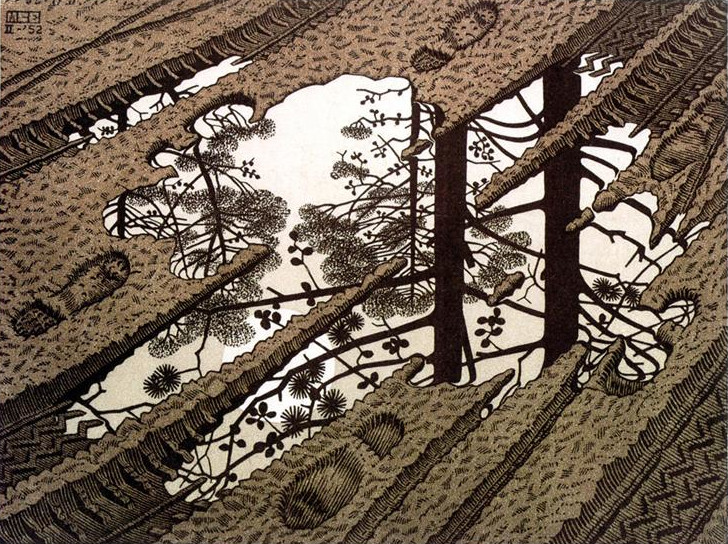
\includegraphics[width=0.9\textwidth]{puddle}
\end{figure}

\vfill

\end{document}
